\documentclass[12pt]{article}
\usepackage[utf8]{inputenc}
\usepackage{graphics}
\usepackage{graphicx}
\usepackage{float}
\usepackage{hyperref}
\hypersetup{
	colorlinks=true,
	linkcolor=blue,
	filecolor=magenta,      
	urlcolor=cyan,
}

\title{De dynamische softwarekwaliteit meten}
\author{Thomas van Dongen, Koen Schilders}
\date{12 april 2018}

\begin{document}


% De titelpagina
\begin{titlepage}
\maketitle
\end{titlepage}

\section{Inleiding}
% Naast statische softwarekwaliteit ook dynamisch kwaliteit testen
% Typen tests:
%	* Performance tests
%	* Resourceverbruik
%	* 

% We gaan de volgende dynamische tests integreren
%	* JUnit in Jenkins
%	* CLIF in Jenkins

% Verder nog advies
%	* Testteam opzetten

Tot nu toe hebben we alleen de statische softwarekwaliteit gemeten, waarmee we kunnen meten wat de kwaliteit van de code is. Maar een applicatie kan alleen werken als de code uitgevoerd wordt, en de code kan tijdens het uitvoeren fouten tonen welke niet afgevangen kunnen worden door statische kwaliteit-checks. Daarom is het noodzakelijk om de dynamische softwarekwaliteit te meten. Dynamisch kwaliteit meten omvat alle tests die door middel van executie uitgevoerd worden, zoals performance- en resourceverbruik meten.
Het is belangrijk om de dynamische softwarekwaliteit te meten. Door te meten kun je te weten komen of je applicatie functioneert wanneer deze draait, en of de applicatie voldoet aan opgestelde niet-functionele requirements. Ook kun je testen hoe de applicatie omgaat met piekmomenten. Dit voorkomt dat een onstabiele applicatie draait op de productieomgeving, met alle nadelige gevolgen van dien.


\section{Dynamische kwaliteit testen}
Er zijn verschillende manieren om de dynamische kwaliteit van een applicatie te testen. In dit project gaan we de uitvoersnelheid van de code testen. Dit kan door middel van JUnit-tests. We hebben al enkele JUnit-tests voor onze Calculator-applicatie. De rekenmachine heeft vier methoden om te testen: add, subtract, multiply en divide. Om de werking van de rekenmachine te garanderen hebben we hier JUnit-tests voor geschreven. Het is alleen niet handig als de methoden te lang doen over het uitrekenen. Door @Test boven de JUnit-test te veranderen in @Test(timeout = 50) wordt de test afgekeurd als deze langer als 50 milliseconden duurt.

\begin{figure}[H]
	\begin{center}
		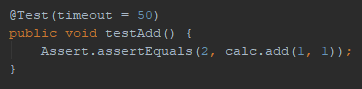
\includegraphics[width=0.75\textwidth]{images/junit_test.png}
		\caption{De JUnit-test met de timeout\label{fig:junit_test}}
	\end{center}
\end{figure}

\subsection{Testteam}
Daarnaast kan het handig zijn een testteam samen te stellen, vooral bij complexe applicaties zoals games. Omdat de testers mensen zijn kunnen ze de applicatie op een menselijke manier testen en actueel gebruik door gebruikers nabootsen. Zo kunnen testers dus naast bugs ook gebruiksvriendelijkheid van de applicatie testen, wat van groot belang is voor applicaties met veel gebruikers.

Het nadeel van een menselijk testteam is dat het veel geld kost, vooral voor lange tijd. Een ontwikkelstraat opzetten is een eenmalige investering welke zich binnen korte tijd terugverdient. Toch kan een testteam de applicatie op een manier testen wat niet te automatiseren is. Het meest voor de hand liggende voorbeeld is het testen van games, welke tot op heden nog steeds met testteams worden getest.

\end{document}